\documentclass[12pt]{report}

\usepackage[T1]{fontenc}
\usepackage[utf8]{inputenc}
\usepackage{graphicx}
\usepackage{amsmath,amssymb,amsfonts}
\usepackage{txfonts}
\usepackage{pdfpages}
\usepackage{caption}
\usepackage{float}

\renewcommand{\chaptername}{Rozdział}
\renewcommand{\contentsname}{Spis treści}
\renewcommand{\figurename}{Rys.}
\renewcommand{\tablename}{Tab.}
\renewcommand{\listfigurename}{Spis rysunków}
\renewcommand{\listtablename}{Spis tabel}
\renewcommand{\bibname}{Bibliografia}

\pagestyle{headings}

\setlength{\textwidth}{14cm}
\setlength{\textheight}{20cm}

\newtheorem{definition}{Definicja}
\newtheorem{example}{Przykład}[chapter]
\newtheorem{corollary}{Wniosek}[chapter]

\begin{document}

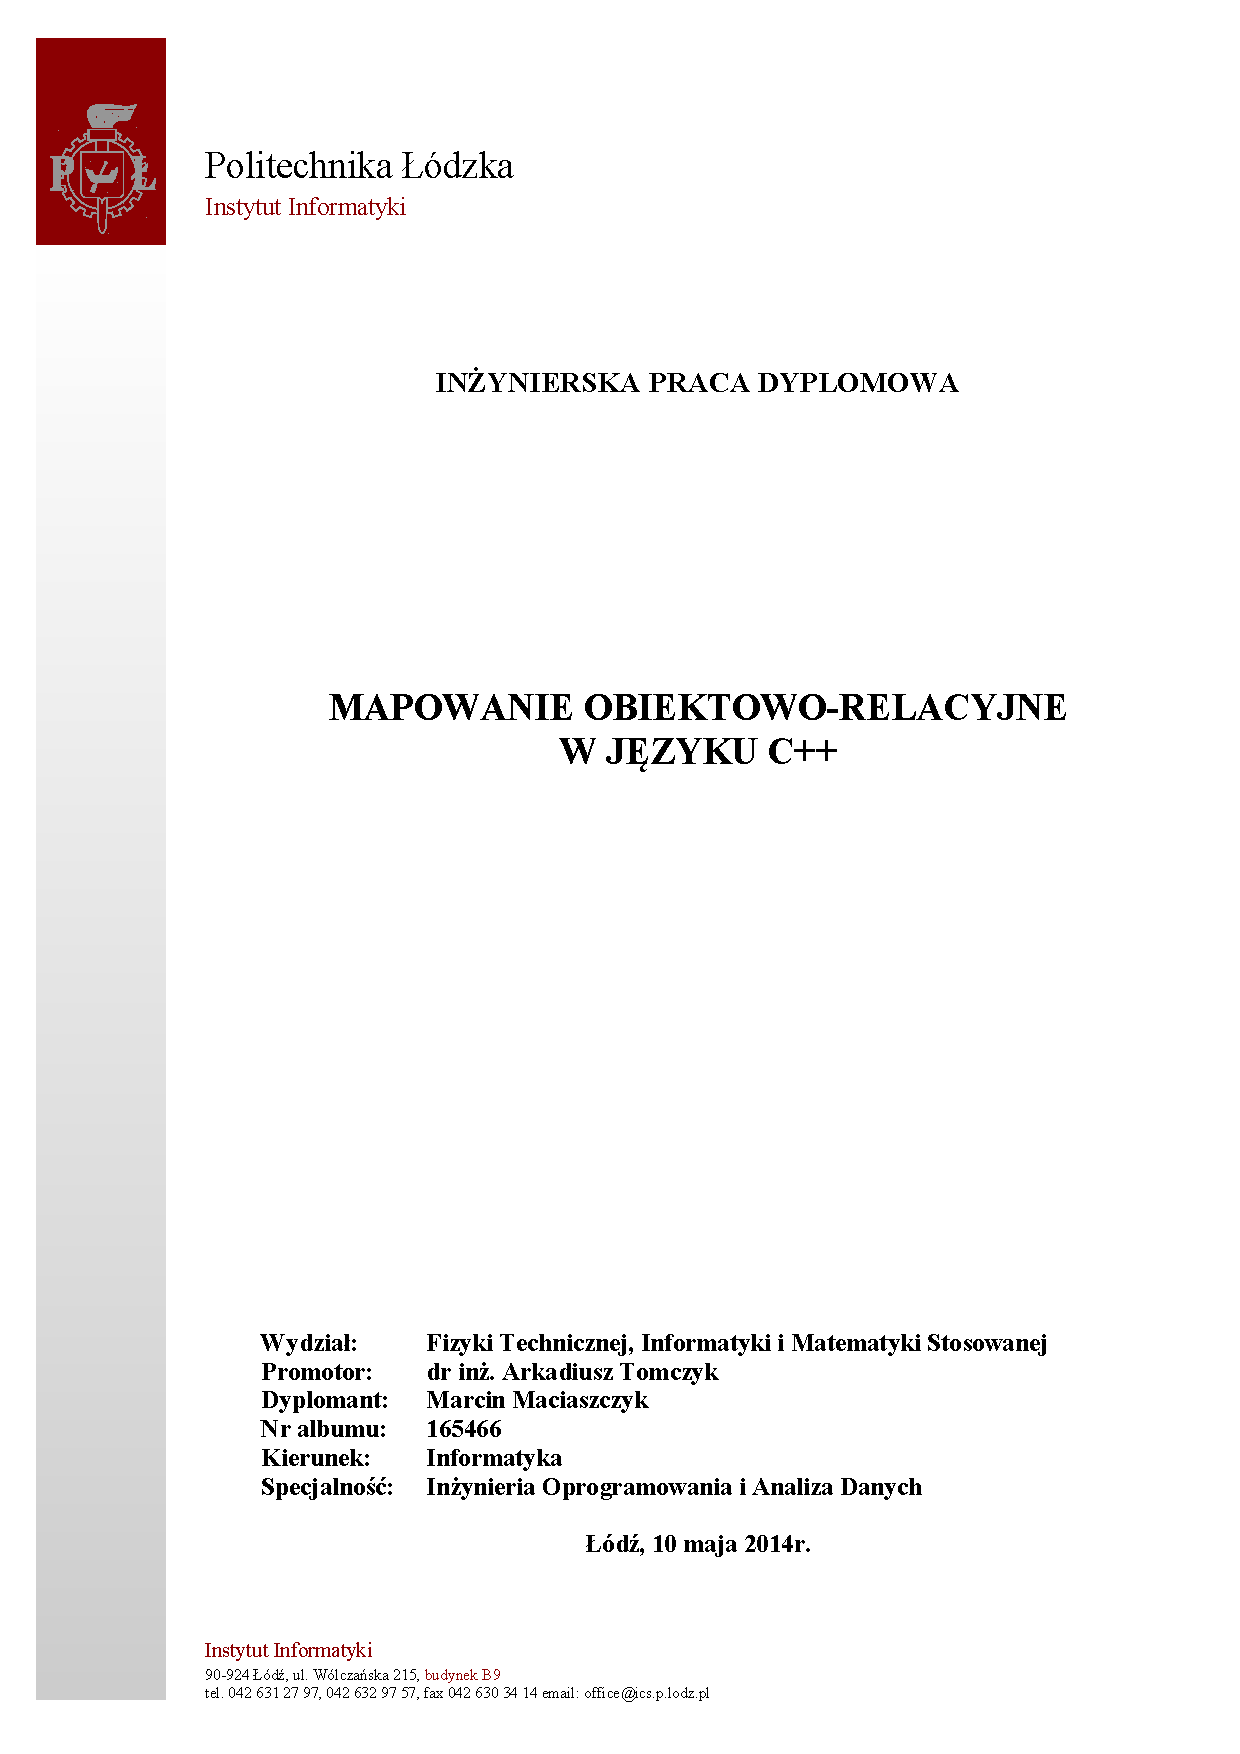
\includepdf[pages={1}]{resources/title_page.pdf}

\tableofcontents

\chapter{Wstęp}
\label{wstep}

\section{Uzasadnienie wyboru tematu}

Wraz z rozwojem informatyki proces tworzenia oprogramowania wymaga od informatyków co raz większej wiedzy w poszczególnych dziedzinach takich jak na przykład bazy 
danych czy sieci komputerowe. Ciężko jest być specjalistą w każdej z nich, dlatego też podczas tworzenia oprogramowania programiści co raz częściej sięgają po różnego 
rodzaju narzędzia programistyczne, które mają za zadanie ułatwić im pracę wykonując jej część za nich.

Przykładem takich narzędzi są aplikacje szkieletowe wykorzystywane jako fundamenty dla tworzonych aplikacji czy też biblioteki programistyczne udostępniające zestawy 
określonych funkcji. Oczywiście nie zawsze mamy możliwość skorzystania z wspominanych narzędzi, jednak jeśli taka istnieje warto wziąć to pod uwagę podczas fazy planowania 
tworzenia  oprogramowania, ponieważ decydując się na korzystanie z nich jesteśmy w stanie zaoszczędzić sporo czasu, a także uniknąć wielu błędów związanych z nieznajomością 
danej dziedziny.

Wraz z kolegą z tego samego roku studiów -- Sebastianem Florkiem, zdecydowaliśmy się w ramach pisamia pracy dyplomowej na wspólne stworzenie aplikacji szkieletowej, 
która będzie realizowała mapowanie obiektowo-relacyjne w języku C++. Wybór C++ jako języka programowania tłumaczymy dość dobrą jego znajomością, a także pewnym
doświadczeniem w programowaniu w tym języku nabytym w trakcie studiów. Mapowanie obiektowo-relacyjne jest to obecnie zagadnienie co raz bardziej powszechne, szczególnie w 
językach programowania takich jak PHP czy Java. Programiści C++ nie mają już tak dużego wyboru wśród dostępnych narzędzi służących do mapowania 
obiektowo-relacyjnego, co także braliśmy pod uwagę ustalając temat nad jakim będziemy pracować.

\begin{figure}[H]
\centering
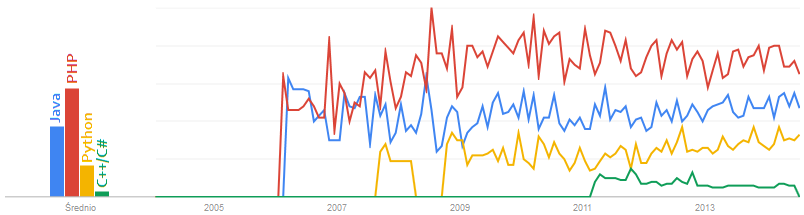
\includegraphics[width=\textwidth]{resources/trends.png}
\caption[Wykres przedstawiający popularność mapowania obiektowo-relacyjnego na przestrzeni czasu w wybranych językach programowania] {Wykres przedstawiający 
popularność mapowania obiektowo-relacyjnego na przestrzeni czasu w wybranych językach programowania \cite{trends}}
\end{figure}

Podział naszej pracy zostanie opisany na początku rozdziału \ref{qubic}, jednak na wstępie warto zaznaczyć, że tematem pracy Sebastiana jest generator opisu mapowania 
obiektowo-relacyjnego, który jest wstępnym etapem pracy naszej aplikacji szkieletowej. Celem wspomnianego generatora jest wygenerowanie pliku projektu, a także plików
nagłówkowych oraz klas na podstawie istniejącej już bazy danych. Moim zadaniem będzie samo mapowanie obiektowo-relacyjne, które będzie się opierało na wcześniej
wygenerowanych plikach. 

\begin{figure}[h]
\centering
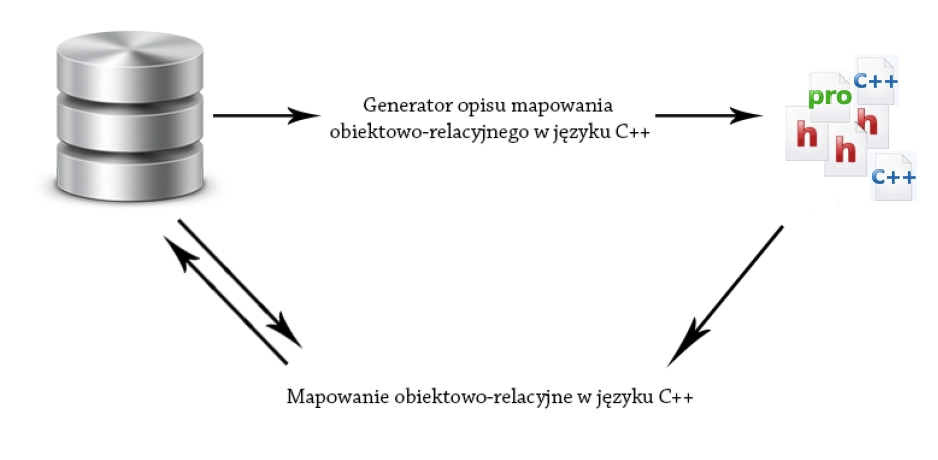
\includegraphics[width=\textwidth]{resources/coop.png}
\caption[Schemat współpracy modułów tworzonej aplikacji szkieletowej]{Schemat współpracy modułów tworzonej aplikacji szkieletowej, dalej występującej też pod nazwą Qubic}
\end{figure}

\section{Problematyka i zakres pracy}

Programowanie obiektowe jest obecnie jednym z najpopularniejszych pa\-ra\-dy\-gma\-tów programowania, a pojęcia takie jak klasa czy obiekt znane są wszystkim programistom.
Podobnie jest z relacyjnym modelem organizacji baz danych i terminami takimi jak relacja czy krotka. Chcąc wykorzystać oba te podejścia w jednej aplikacji musimy zadbać o 
obustronną konwersję pomiędzy danymi z tabel relacyjnej bazy danych a obiektami aplikacjii. Tym właśnie zajmuje się mapowanie obiektowo-relacyjne, które wraz z tworzeniem 
aplikacji szkieletowych w języku C++ jest główną problematyką niniejszej pracy.

Tutaj powstaje pytanie czy na prawdę warto korzystać z bibliotek i aplikacji szkieletowych służących do mapowania obiektowo relacyjnego? Od\-po\-wiedź nie jest
jednoznaczna w wszystkich przypadkach, ale warto wymienić jego podstawowe wady i zalety, których dokładniejsza analiza znajduje się w dalszej części pracy. Zacznijmy od zalet 
wykorzystania narzędzi ORM\footnote{~mapowanie obiektowo-relacyjne (ang. Object-Relational Mapping)}:

\begin{itemize}
\item Znacznie zredukowana ilość pracy wymagana na oprogramowanie dostępu do bazy danych.
\item Nieobowiązkowa znajomość języka SQL\footnote{~strukturalny język zapytań (ang. Structured Query Language)}. W celu tworzenia zapytań do bazy
danych korzystamy z interfejsu udostępnianego przez daną bibliotekę czy też aplikację szkieletową.
\item Uniezależnienie się od rodzaju systemu zarządzania bazą danych, możemy korzystać równie dobrze z MySQL, Oracle, PostgreSQL czy też Microsoft SQL Server
niekoniecznie posiadając o nich rozbudowaną wiedzę.
\item Aby skorzystać z transakcji, połączenia z bazą danych a także wieu innych funkcjonalności baz danych wystarczy zazwyczaj wywołać pojedyńczą me\-to\-dę.
\item Cały model danych przechowywany jest w jednym miejscu oraz nie jest ściśle związany z wykorzystywanym systemem zarządzania bazą danych dzięki cze\-mu łatwiej 
jest nam wprowadzać kolejne modyfikacje w kodzie oraz nawet zmieniać system zarządzania bazą danych na inny.
\end{itemize}

Wszędzie gdzie pojawiają się zalety mamy też do czynienia z wadami, nie inaczej jest w tym przypadku:

\begin{itemize}
\item Konfiguracja jest najczęściej skomplikowana i wymaga sporo czasu.
\item Aby efektownie korzystać z narzędzi do mapowania obiektowo-relacyjnego wymagana jest od nas ich dobra znajomość.
\item Proste zapytania są obsługiwane bardzo sprawnie, jednak gdy przetwarzamy duże ilości złożonych zapytań wydajność nie dorówna nigdy zapytaniom na\-pi\-sa\-nym
przez specjalistę znającego język SQL.
\item Abstrakcja wprowadzona przez narzędzia ORM może okazać się uciążliwa, ponieważ nie zawsze zdajemy sobie sprawę z tego co dzieje się za kulisami w trakcie
wykonywania poszczególnch operacji.
\end{itemize}

Naszym głównym celem jest uczynienie Qubica dobrą alternatywą dla nie\-li\-cznych, ale istniejących już bibliotek oraz aplikacji szkieletowych realizujących mapowanie 
obiektowo-relacyjne w języku C++. Wszystkie nam obecnie znane rozwiązania są dostępne za darmo, jednak nie udostępniają one generatora opisu będącego w stanie 
wygenerować cały projekt aplikacji a ich interfejsy nie należą do intuicyjnych. Wprowadzenie generatora oraz intuicyjnego interfejsu użytkownika powinno uczynić Qubica
istotną alternatywą dla istniejących już narzędzi za\-kła\-da\-jąc, że pozostała funkcjonalność mapowania obiektowo-relacyjnego zostanie zre\-al\-iz\-owana poprawnie.

Analizę istniejących rozwiązań przedstawia kolejny rozdział a zestawienie z rezultatami naszej pracy znajduje się natomiast w końcowej części pracy, gdzie zostaną
przedstawione uzyskane przez nas wyniki oraz podsumowanie wykonanej przez nas pracy.

\section{Cele pracy} % Podrozdział około 1 strony, czyli 1800 znaków. Każdy cel opisany w 2-3 zdaniach, bez używania skrótów.

Do najważniejszych celów niniejszej pracy dyplomowej należą:

\begin{itemize}
\item Analiza istniejących bibliotek oraz aplikacji szkieletowych realizujących ma\-po\-wa\-nie obiektowo-relacyjne w języku C++ -- przeanalizowanie istniejących już narzędzi
umożliwi dokładniejsze zapoznanie się z tematyką mapowania obiektowo-relacyjnego a także ze sposobem działania istniejących już rozwiązań, co umożliwi zaczerpnięcie 
najciekawszych pomysłów dla Qubica a także wskaże elementy, które mogą ulec w nim poprawie.
\item Stworzenie własnej aplikacji szkieletowej realizującej mapowanie obiektowo-relacyjne w języku C++ -- ułatwi dokładniejsze poznanie mechanizmów dzia\-łających
podczas mapowania obiektowo-relacyjnego oraz sposobów ro\-zwią\-zania pojawiających się problemów.

\item Porównanie szybkości działania oraz ilości kodu wymaganego do stworzenia przykładowej aplikacji stworzonej w oparciu o Qubic a o inne istniejące na\-rzędzia -- 
przeprowadzenie testów pozwoli stwierdzić czy przyjęte założenia i zastosowane rozwiązania wpłynęły na stworzenie wartej uwagi aplikacji szkieletowej realizującej
mapowanie obiektowo-relacyjne.
\end{itemize}

Do celów części praktycznej należą:

\begin{itemize}
\item Stworzenie intuicyjnego interfejsu użytkownika -- aby sprawdzić w jakim stopniu udało się zrealizować założenia zostanie przeprowadzony test po\-le\-ga\-ją\-cy na 
napisaniu tej samej aplikacji wykorzystującej Qubica oraz inne aplikacje szkieletowe i bibioteki, a następnie porównaniu ilości linii kodu stworzonych aplikacji.
\item Stworzenie generatora opisu mapowania obiektowo-relacyjnego -- jest to przed\-mio\-tem pracy Sebastiana, naszym wspólnym celem jest integracja obu modułów.
\item Poprawne zrealizowanie założeń mapowania obiektowo-relacyjnego, a także jak najlepsza optymalizacja zapytań -- aby sprawdzić w jakim stopniu udało się zrealizować
założenia zostanie przeprowadzony test polegający na napisaniu tej samej aplikacji wykorzystującej Qubica oraz inne aplikacje szkieletowe i bibioteki, a następnie porównaniu
ich wydajności.
\item Uczynienie konfiguracji Qubica jak najprostszą.
\end{itemize}

\section{Metoda badawcza}

\subsection{Studia literaturowe}

Literatura wykorzystana podczas pisania niniejszej pracy dotyczy głównie czterech zagadnień, czyli tworzenia aplikacji szkieletowych w języku C++, tworzenia zapytań w 
języku SQL, aplikacji szkieletowej Qt oraz mapowania obiektowo-relacyjnego. Pierwsze dwa należą są dość popularne, dlatego też wybór pozycji książkowych jest dość spory. 
Na temat mapowania obiektowo-relacyjnego trudniej jednak znaleźć podobną ilość książek, jednak istnieje spora ilość artykułów w wersji elektronicznej. Najczęściej są one
napisane w języku angielskim. Tytuły wykorzystanych pozycji bibliograficznych wraz z ich krótkimi opisami znajdują się w kolejnym rozdziale.

\subsection{Analiza istniejących rozwiązań}

Poza podstawowym źródłem informacji jakim są studia literaturowe podczas pisania tej pracy przeprowadzona została analiza istniejących już narzędzi realizujących mapowanie
obiektowo-relacyjne. Analiza taka umożliwia poznanie praktycznych rozwiązań problemów pojawiających się podczas prac badawczych nad daną tema\-tyką.

\subsection{Stworzenie własnej aplikacji szkieletowej}

Praktyka jest najczęściej najlepszą z dostępnych metod nauki i to właśnie podczas tworzenia własnej aplikacji szkieletowej realizującej mapowanie obiektowo-relacyjne można
się najbardziej z danym tematem zapoznać. Wszystkie problemy, które pojawiały się poczas pisania Qubica musiały zostać w pewien sposób roz\-wią\-zane i to właśnie analiza
tych problemów i ich rozwiązywanie było główną metodą badawczą wykorzystaną podczas pisania niniejszej pracy.

\subsection{Analiza porównawcza oraz testy}

Analizując wcześniej istniejące już rozwiązania i powównując je z własnym można dojść do najtrafniejszych wniosków. To właśnie na tym etapie często dowiadujemy się czy
przyjęte przez nas założenia i zaproponowane rozwiązania były lepsze niż te z istniejących już rozwiązań. 

\section{Przegląd literatury w dziedzinie}

\subsection{Literatura dotycząca języka C++ oraz Qt}

W celu zasięgnięcia informacji na temat języka C++ i zagadnień z nim związanych najczęściej wykorzystywaną pozycją książkową była ,,Symfonia'' Jerzego Grębosza \cite{symfonia}.
Najlepszym jej określeniem jest ,,kurs programowania w języku C++'', opisane zostały w niej jednak zagadnienia dotyczące nie tylko języka C++, a także co istotne dla
autora niniejszej pracy zagadnienia dotyczące obiektowości.

Poza tym wartościowym źródłem wiedzy podczas tworzenia Qubica była specyfikacja języka C++ \cite{cpp} oraz dokumentacja aplikacji szkieletowej Qt \cite{qt}.

\subsection{Literatura dotycząca języka SQL}

Kluczowym zadaniem Qubica jest tworzenie jak najefektywniejszych zapytań w języku SQL, wiedza autora na ten temat pochodzi w głównej mierze z książki Johna Viescasa o
tytule ,,SQL Queries for Mere Mortals'' \cite{sql}. Wyjaśnione zostały w niej zagadnienia dotyczące tworzenia zapytań w języku SQL oraz podstawy związane z bazami danych.

W tym przypadku także wartościowe okazały się specyfikacje na przykład języka MySQL \cite{mysql}.

\subsection{Literatura dotycząca mapowania obiektowo-relacyjnego}

Głównym źródłem wiedzy autora na temat mapowania obiektowo-relacyjnego były źródła elektroniczne, do których zaliczają się przede wszyskim artykuły naukowe. Odniesienia
do tych artykułów znajdują się głównie w rozdziale /ref{teoria}, gdzie pojęcia dotyczące mapowania są objaśniane.

\section{Układ pracy} % Cały podrozdział około 1 strony.

Tematem niniejszej pracy jest mapowanie obiektowo-relacyjne w języku C++, zaś za jej główny cel przyjęto przeanalizowanie istniejących bibliotek oraz aplikacji szkieletowych
realizujących mapowanie obiektowo-relacyjne oraz stworzenie własnej aplikacji szkieletowej.

Najważniejszym celem pracy jest przeanalizowanie istniejących narzędzi służących do mapowania obiektowo-relacyjnego w języku C++ oraz stworzenie na podstawie tej analizy
własnej aplikacji szkieletowej realizującej to samo zagadnienie.

Rodział \ref{wstep} otwiera uzasadnienie wyboru tematu pracy, opisane zostały w nim także cele pracy, jej problematyka, zakres, wykorzystane metody badawcze, prze\-gląd 
literatury oraz jej układ.

Rozdział \ref{teoria} zawiera objaśnienia podstawowych zagadnień teotetycznych związanych z mapowaniem obiektowo-relacyjnym oraz tworzeniem aplikacji szkieletowych w
języku C++.

Rozdział \ref{analiza} przedstawia analizę istniejących już narzędzi służących do mapowania obiektowo-relacyjnego napisanych w języku C++.

Rozdział \ref{qubic} przedstawia projekt aplikacji szkieletowej Qubic, postawione wymagania, opis jego implementacji, wyniki testów oraz końcowe porównanie z wcześniej
analizowanymi narzędziami w rozdziale \ref{analiza}.

Rozdział \ref{podsumowanie} zawiera podsumowanie niniejszej pracy inżynierskiej, biorąc pod szczególną uwagę dyskusję wyników oraz dalsze prespektywy rozwoju pracy.

\chapter[Zagadnienia teoretyczne]{Zagadnienia teoretyczne dotyczące mapowania obiektowo-relacyjnego oraz aplikacji szkieletowych}
\label{teoria}

\section{Programowanie obiektowe}

\section{Relacyjne bazy danych}

\section{Mapowanie obiektowo-relacyjne}

\chapter[Analiza istniejących rozwiązań]{Analiza istniejących rozwiązań mapowania obiektowo-relacyjnego w języku C++}
\label{analiza}

\section{Przegląd istniejących rozwiązań}

\section{Porównanie istniejących rozwiązań}

\begin{table}[h]
\centering
\begin{tabular}{| l | l | l | l | l |} 
\hline 
Nazwa & QxOrm & Debea & SOCI & OpenORM \\ \hline
Typ & - & - & - & - \\ \hline
Cena & 0 zł & 0 zł & 0 zł & 0 zł \\ \hline
Obsługiwane bazy & - & - & - & -  \\ \hline
\end{tabular} 
\caption{Porównanie istniejących rozwiązań}
\end{table}

\chapter{Aplikacja szkieletowa Qubic}
\label{qubic}

\section{Moduły tworzonej aplikacji}

W rozdziale pierwszym w skrócie został przedstawiony schemat współpracy modułu tworzonego przez autora tej pracy a autora pracy, której tematem jest ,,Generator opis
mapowania obiektowo-relacyjnego w języku C++''. W tym podrozdziale opis ten zostanie rozwinięty.

Chcąc w jak największym stopniu zautomatyzować obsługę połączenia z bazą oraz zminimalizować czas jaki programista będzie musiał poświęcić na oprogra\-mowywanie
komunikacji pomiędzy programem a bazą danych zdecydowaliśmy się na wprowadzenie generatora opisu, który tę część pracy wykona za użytkownika Qubica.

Zadaniem generatora jest wygenerowanie plików klas, plików nagłówkowych oraz pliku projektu Qt w oparciu o istniejącą bazę danych. Moduł tworzony przez autora niniejszej
pracy będzie wykorzystywany w wygenerowanym kodzie, a także w kodzie napisanym przez użytkownika Qubica. W momencie zakończenia pracy generatora wygenerowana
aplikacja będzie w pełni gotowa do przechowywania danych z bazie bez konieczności tworzenia zapytań. W celu przechowania obiektów aplikacji, ich modifikacji, załadowania 
czy usunięcia z bazy danych wystarczy uruchomienie odpowiednich metod Qubica.

Dalsza część tego rozdziału została poświęcona w zdecydowanej większości modułowi Qubica zajmującego się mapowaniem obiektowo-relacyjnym.

\section{Analiza wymagań}

\subsection{Wymagania funkcjonalne}

Podczas projektowania Qubica przyjęto następujące założenia w celu jak najlepszego odwzorowania cech mapowania obiektowo-relacyjnego:

\begin{itemize}
\item Aplikacja musi umożliwiać podstawowe operacje mapowania obiektowo-rela\-cyjnego, a więc zapisywanie obiektów do bazy danych, ich odczyt, aktualizowanie obiektów
już zapsanych w bazie oraz ich usuwanie.
\item Aplikacja musi udostępniać interfejs do tworzenia zapytań z poziomu kodu, dzięki temu jej użytkownik nie musi znać języka SQL.
\item Aplikacja musi udostępniać funkcje dostępu do powiązanych danych w przypadku wystąpienia relacji różnych od jeden do jednego. Użytkownik powinien mieć możliwość
uzyskania dostępu do obiektów powiązanych z wybranym obiektem bez konieczności własnoręcznego konstruowania zapytań.
\item Aplikacja powinna posiadać wsparcie dla wielu rodzajów baz danych, ewentualnie musi być ona łatwo rozszerzalna.
\item Aplikacja musi posiadać możliwość wykorzystania transakcji.
\item Aplikacja musi posiadać możliwość konfiguracji.
\end{itemize}

\subsection{Wymagania niefunkcjonalne}

Do wymagań niefunkcjonalnych postawionych projektowanej aplikacji należą:

\begin{itemize}
\item Użytkowanie aplikacji powinno być jak najbardziej intuicyjne, co za tym idzie kod użytkownika mający za zadanie wykonywać podstawowe operacje powinien zajmować
jak najmniej linii.
\item Aplikacja musi działać możliwie szybko, czas podstawowych operacji nie powinien znacząco odbiegać od tego w przypadku gdy użytkownik sam two\-rzyłby zapytania do bazy.
\item Aplikacja musi rozpoznawać relacje jeden do jednego, jeden do wielu oraz wiele do wielu i odpowiednio je obsługiwać.
\item Pamięć w trakcie działania aplikacji musi być odpowiednio zarządzana, niedopuszczalne są żadne wycieki pamięci czy też zapętlenia się programu.
\item Błędy pojawiające się w trakcie działania aplikacji powinny być prawidłowo obsługiwane i sygnalizowane użytkownikowi.
\end{itemize}

\section{Projekt}

\subsection{Rodzaj aplikacji}

Qubic jest aplikacją szkieletową, czyli strukturą do wykorzystywaną do budowy innych aplikacji. Jego podstawowym zadaniem jest realizacja mapowania obiektowo-relacyjnego,
czyli udostępnienie funkcjonalności pozwalającej na przechowywanie obiektów w bazie danych.

W celu stworzenia aplikacji w oparciu o Qubica użytkownik musi przygotować bazę danych na podstawie której wygenerowany zostanie plik projektu Qt wraz z plikami nagłówkowymi
oraz plikami klas. W tym momencie aplikacja posiada już oprogramowany dostęp do danych i użytkownik może zająć się implementowaniem własnej logiki czy też warstwy widoku.

\subsection{Diagram klas}

Diagram klas Qubica przedstawia rysunek \ref{diagram}:

\newpage
\noindent
\begin{minipage}{\linewidth}
\makebox[\linewidth]{
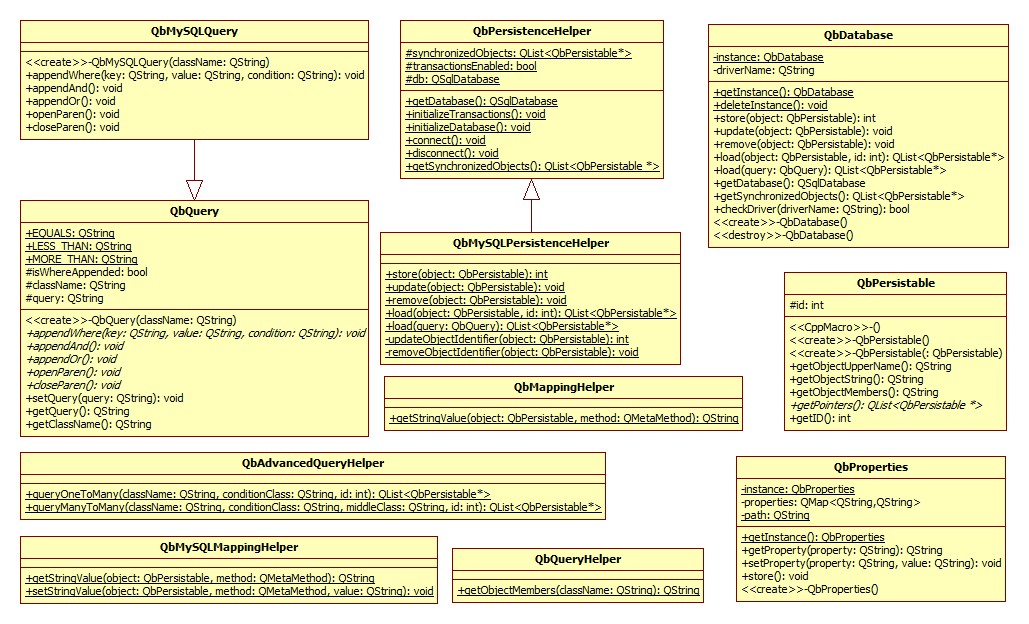
\includegraphics[keepaspectratio=true, width=.9\textwidth]{resources/diagram.jpeg}}
\captionof{figure}{Diagram klas}
\label{diagram}
\end{minipage}

\subsection{Wzorce projektowe}

Jednym z wzorców projektowych, które znalazły zastosowanie w Qubicu jest Singleton. Do jego największych zalet należy fakt, że klasa go wykorzystująca może posiadać 
co najwyżej jedną instancję do której istnieje globalny dostęp. Singleton swoje zastosowanie znajduje w przypadku gdy programista chce ograniczyć liczbę instancji dla 
wybranych klas a także samemu odpowiadać za ich tworzenie. W przypadku Qubica został on wykorzystany w klasach {\tt QbDatabase} oraz {\tt QbProperties}. Tworzenie 
więcej niż jednej instancji tych klas nie ma sensu biorąc pod uwagę specyfikę projektu, więc najlepszym rozwiązaniem wydaje się być zablokowanie tej możliwości użytkownikowi. 

\subsection{Środowisko programistyczne}

Qubic został napisany w języku C++ w oparciu o aplikację szkieletową Qt, co za tym idzie wybór platformy należy do użytkownika i równie dobrze może to być Windows jak i Linux.
Zarówno wybór bazy danych nie został narzucony z góry, co prawda na potrzeby projektu zaimplementowana została obsługa tylko dla bazy MySQL jednak zapewniona została 
łatwa rozszerzalność i dodanie obsługi dla innych rodzajów baz danych nie powinna być problemem.

Jedyną biblioteką wykorzystywaną przez Qubica jest QsLogger odpowiedzialny za logowanie. Jest to bardzo przydatna funkcja, która umożliwia szybkie zlokalizowanie pojawiających
się problemów.

\subsection{System kontroli wersji}

Podczas pracy nad projektami w których bierze udział więcej niż jedna osoba bardzo dobrym rozwiązaniem jest korzystanie z systemów kontroli wersji. Ułatwiają one wspólną
pracę oraz organizację tworzonych projektów.

Wybór autorów Qubica padł na dobrze znany serwis GitHub\footnote{~oficjalna strona serwisu -- \tt https://github.com/}. Poza repozytorium na którym znaleźć można kod 
źródłowy Qubica podczas implementacji projektu wykorzystany został system Issues and Milestones\footnote{~problemy oraz kamienie miliowe}, który ułatwia organizację pracy 
nad projektem.

\begin{figure}[h]
\centering
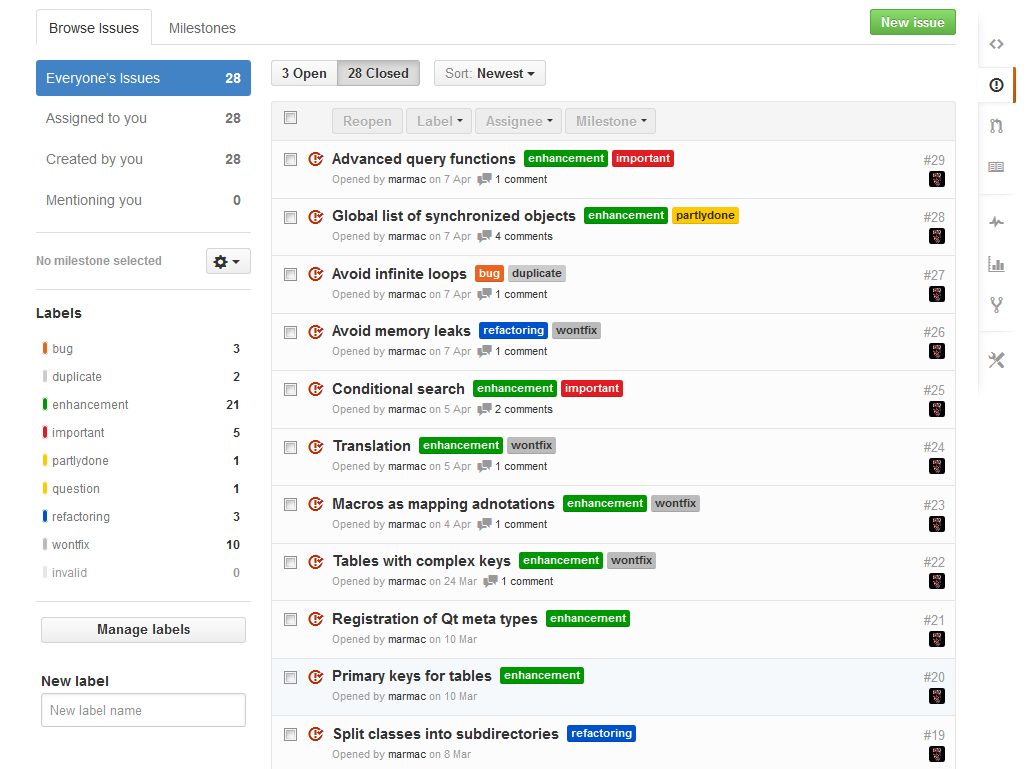
\includegraphics[width=\textwidth]{resources/githubissue.png}
\caption{Przejrzysty widok systemu GitHub Issues}
\end{figure}

\begin{figure}[h!]
\centering
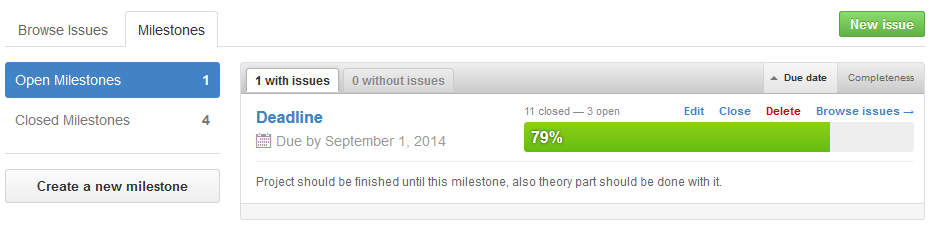
\includegraphics[width=\textwidth]{resources/githubmilestone.png}
\caption{Przejrzysty widok systemu GitHub Miletsones}
\end{figure}

\section{Implementacja}

\subsection{Interfejs CRUD}

Kluczowym modułem narzędzi programistycznych realizujących mapowanie obiekt\-owo-relacyjne jest interfejs CRUD umożliwiający manipulowanie danymi w bazie danych z 
poziomu kodu. Interfejs ten dostępny jest w podstaci co najmniej czterech metod, które jako argumenty przyjmują obiekty dziedziczące po jednej z klas Qubica -- 
{\tt QbPersistable}. Umożliwia to wykorzystanie polimorfizmu, a przecież podczas operacji na obiektach od samego początku nie znany jest dokładny typ obiektu.

Aby mapowanie mogło skutecznie działać potrzebny jest jego jednoznaczny opis, część narzędzi je realizujących korzysta z adnotacji, które określają mapowanie pomiędzy
konkretnymi polami klas a konkretnymi tabelami w bazie danych. W Qubicu problem ten został rozwiązany w trochę inny sposób, który umożliwia stworzony generator opisu
mapowania obiektowo-relacyjnego. Generowane pliki klas są tworzone według ściśle określonych zasad, co oznacza, że nazwy metod dostępowych odpowiadają w pewien
sposób nazwom tabel i ich kolumn. Przykładowo dla kolumny o nazwie {\tt NAME} w tabeli {\tt EMPLOYEE} w pliku klasy {\tt Employee} zostaną wygenerowane metody 
{\tt getName()} oraz {\tt setName(QString name)}. Wie\-dza ta została wykorzystana w trakcie korzystania z mechanizmu refleksji. Konfiguracja samego mapowania nazw
została zapisana w pliku konfiguracyjnym Qubica.

Schematy działania czterech podstawowych metod dostępu przedstawiają po\-niższe schematy blokowe:

\newpage
\begin{figure}[H]
\centering
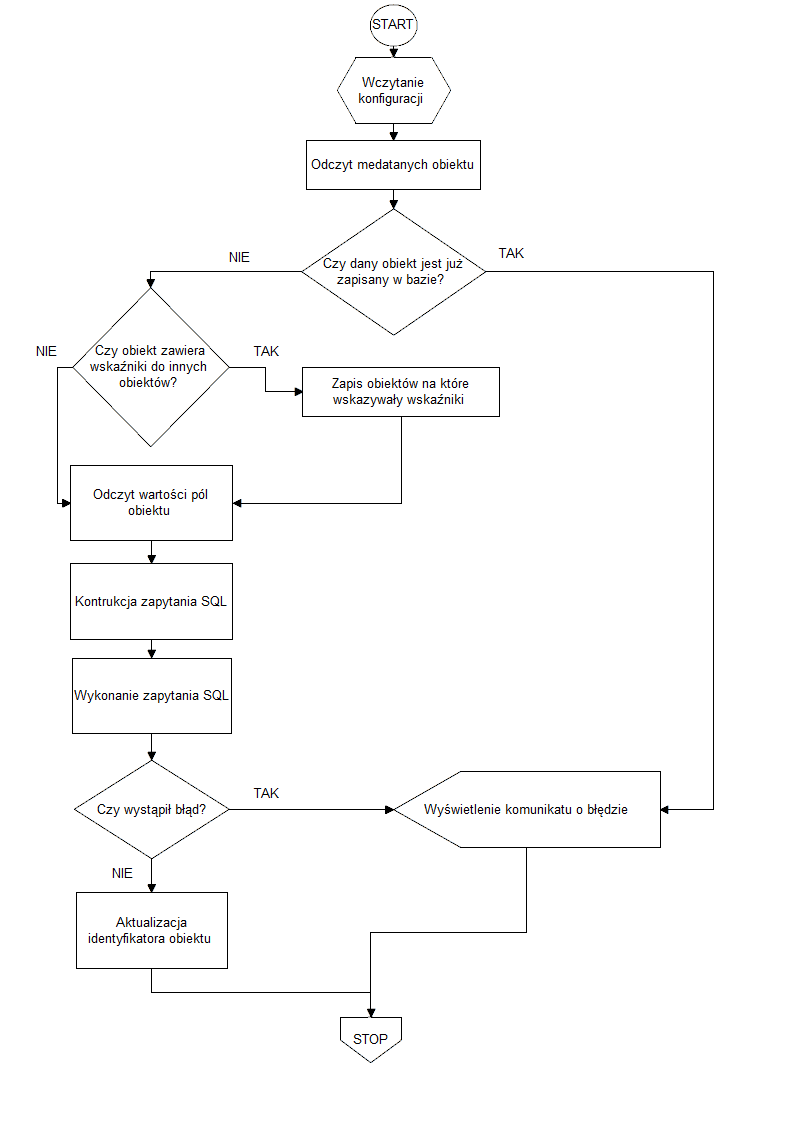
\includegraphics[width=\textwidth]{resources/store_schema.png}
\caption{Schemat blokowy metody zapisującej obiekty w bazie danych}
\end{figure}

\begin{figure}[H]
\centering
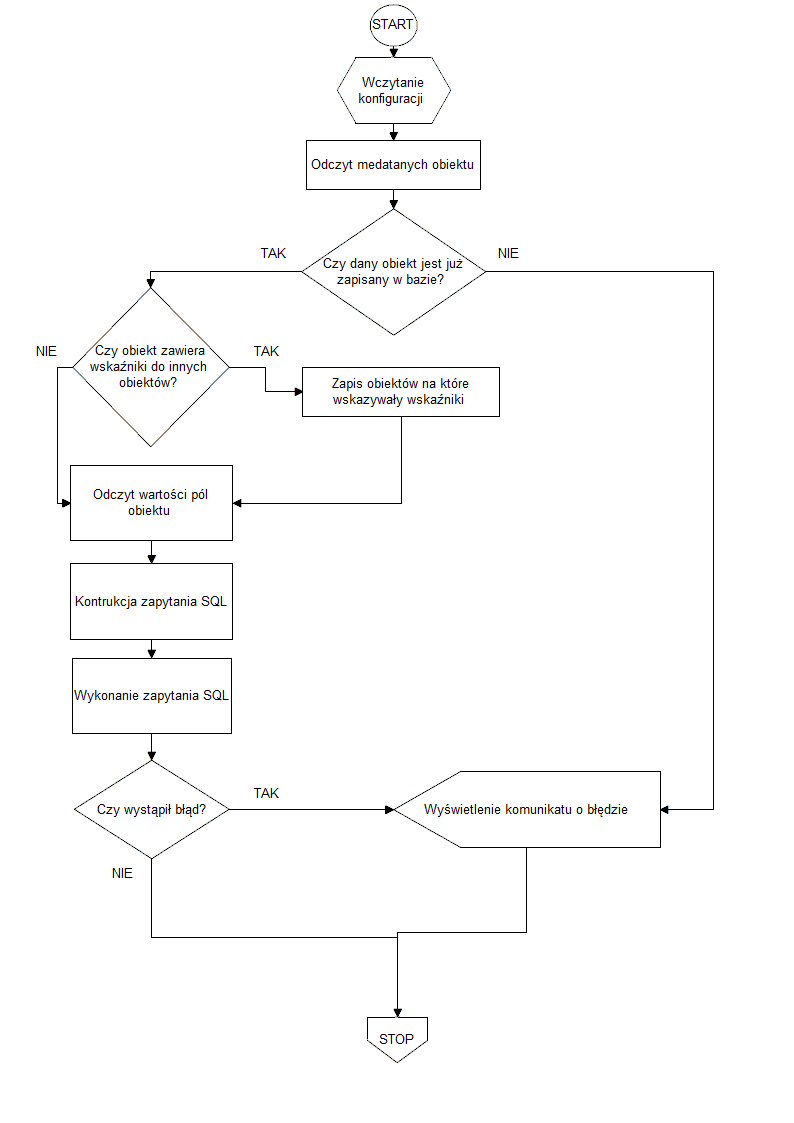
\includegraphics[width=\textwidth]{resources/update_schema.png}
\caption{Schemat blokowy metody aktualizującej obiekty w bazie danych}
\end{figure}

\begin{figure}[H]
\centering
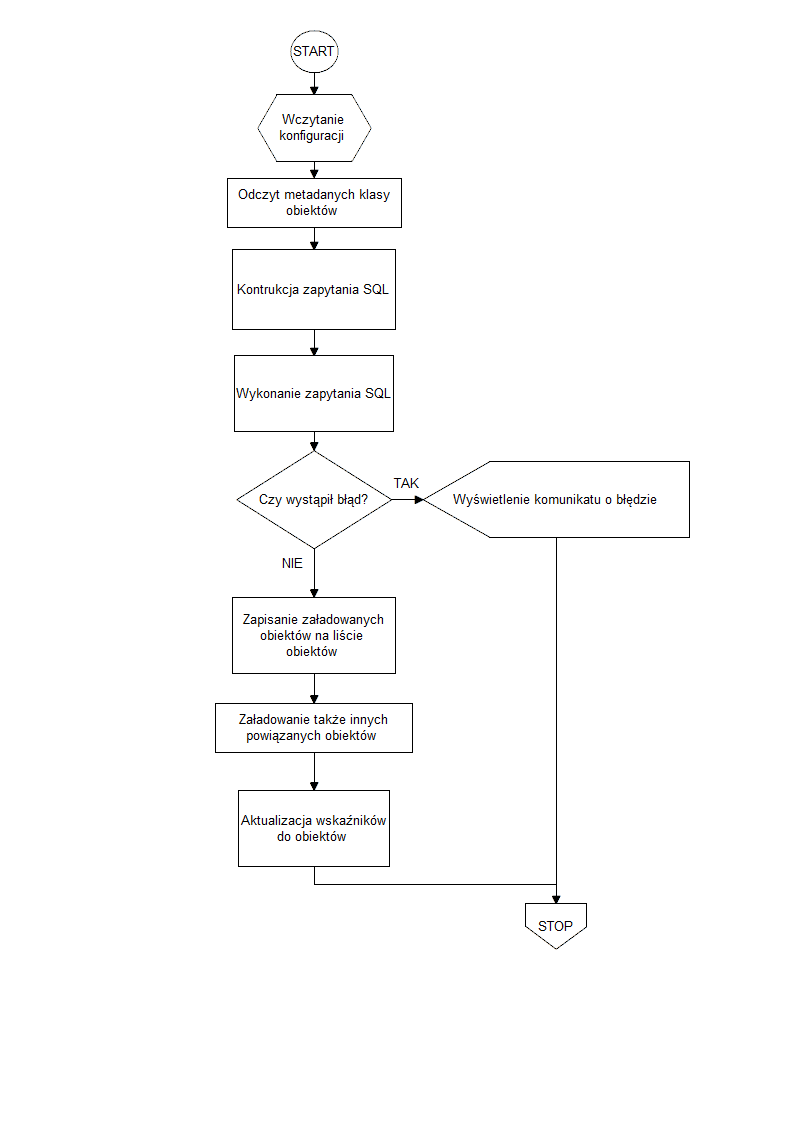
\includegraphics[width=\textwidth]{resources/load_schema.png}
\caption{Schemat blokowy metody ładującej obiekty z bazy danych}
\end{figure}

\begin{figure}[H]
\centering
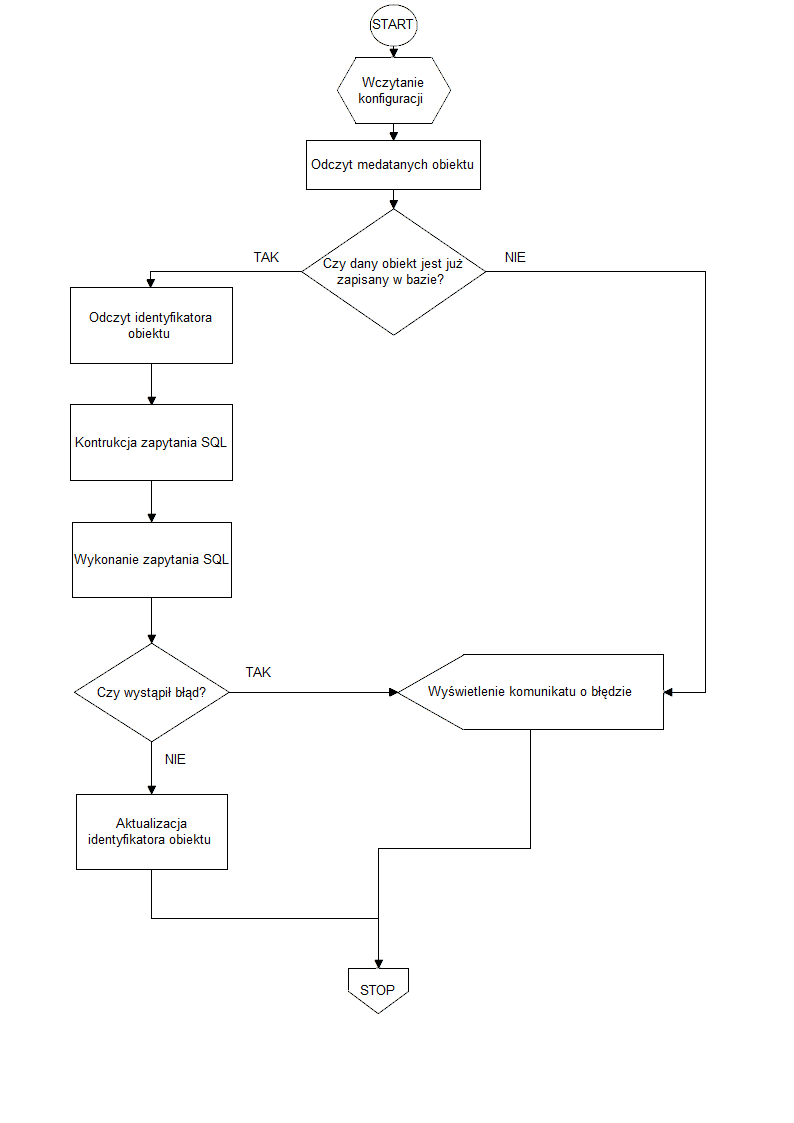
\includegraphics[width=\textwidth]{resources/remove_schema.png}
\caption{Schemat blokowy metody usuwającej obiekty z bazy danych}
\end{figure}

\section{Konserwacja i inżynieria wtórna} %Jak przebiega eksploatacja projektu? Jakie wady i zalety ujawniły się po okresie testowania i użytkowania?
% Jak można skorzystać z tej wiedzy praktycznej pod kątem roz\-bu\-do\-wy pracy? Jakie elementy systemu powinny zostać w pierwszej kolejności zmodyfikowane?  

\section{Dokumentacja użytkownika}

\section{Przykładowa aplikacja wykorzystująca Qubica}

\section{Testy oraz ich wyniki}

\section{Perspektywy rozwoju Qubica}
\label{perspektywyqubic}

W celu dalszego rozwoju stworzonej aplikacji szkieletowej warto rozważyć wprowadzenie następujących usprawnień:

\begin{itemize}
\item System adnotacji -- obecnie na opis mapowania składają się odpowienie nazwy funkcji oraz makra Qt. Istnieje jednak możliwość wprowadzenia własnych makr, które
miałyby opisywać mapowanie pomiędzy nazwami tabel z baz danych a odpowiednimi polami klas napisanych z języku C++. Dzięki temu zaistniałaby możliwość uniezależnienia
nazw pól klas od nazw tabel w bazie danych.
\item Interfejs zapytań -- choć jest już zaimplementowany, nadal nie udostępnia on wszystkich możliwych funkcjonalności języka SQL. Implementacja obsługi takich poleceń
jak JOIN czy UNION z pewnością byłaby dodatkowym atutem.
\item Identyfikacja tabel także za pomocą kluczy złożonych -- w tej chwili tabele identyfikowane są za pomocą kluczów głównych, co z kolei wymusza ich nadawanie w każdej
z tabel.
\item Pamięć podręczna -- wprowadzenie pamięci podręcznej może znacznie polepszyć wydajność w przypadku ciągłych operacji na tych samych danych.
\item Konfiguracja z poziomu kodu -- obecnie większość konfiguracji jest zapisana w plikach konfiguracyjnych i tylko tam może być zmieniana, w celu rozwoju wprowadzenie
dodatkowej możliwości jego konfiguracji wydaje się być dobrym pomysłem.
\item Wsparcie dla różnych rodzajów baz danych -- wprowadzenie tego usprawnienia ogranicza się do implementacji kilku interfejsów dla innych niż MySQL rodzajów baz 
danych. Biorąc pod uwagę możliwość wzorowania się na zaimplementowanej już logice nie powinno to stworzyć problemu gdy zaistnieje taka konieczność.
\item Serializacja danych -- dodanie możliwości serializacji może okazać się użyteczne w przypadku pracy z dużymi ilościami danych, w tym celu można skorzystać z wielu
istniejących już bibliotek udostępniających tę możliwość.
\item Internacjonalizacja -- w tej chwili wszystkie logi zlokalizowane są w języku angielskim, istnieje jednak możliwość zmiany obecnego stanu poprzez wykorzystanie modułu
translacji udostępnianego przez Qt.
\item Wielowątkowość -- wykorzystanie wielowątkowości w przypadku mapowania-obiektowo relacyjnego z pewnością nie należy do najłatwiejszych zadań, jednak znacznie
może to usprawnić wykonywanie bardziej wymagających operacji.
\end{itemize}

\chapter{Podsumowanie}
\label{podsumowanie}

\section{Dyskusja wyników}

\section{Perspektywy rozwoju pracy}

W celu rozwoju niniejszej pracy dyplomowej należy przede wszystkim rozważyć dalsze prace nad stworzoną aplikacją szkieletową. W rozdziale \ref{perspektywyqubic} przedstawione
zostały liczne możliwości rozwoju Qubica, ich realizacja z pewnością byłaby sporym krokiem w przód.

Podjęcie się tego zadania oznaczałoby jednak trzymanie się tematyki mapowania obiektowo-relacyjnego a przecież aplikacja szkieletowa nie musi ograniczać się do realizacji
tylko jednego zagadnienia, istnieje wiele innych możliwości rozwoju. Dobrym tego przykładem jest aplikacja szkieletowa Spring, która oferuje bardzo duże możliwości. Qubic można
rozwijać w podobnym kierunku, zarazem zmieniając główny temat pracy dyplomowej. Nowym tematem mogłaby zostać na przykład aplikacja szkieletowa na telefony
komórkowe czy też aplikacja szkieletowa do tworzenia usług internetowych\footnote{~ang. webservice}.

\addcontentsline{toc}{chapter}{Bibliografia} 
\begin{thebibliography}{99}
\bibitem{trends} Trendy Google. {\tt https://www.google.pl/trends/explore\#q=orm\%20\-java\%2C\%20orm\%20php\%2C\%20orm\%20python\%2C\%20orm\%20c\&cmpt=q}.
\bibitem{symfonia} Grębosz, Jerzy. Symfonia C++. Standard. Wyd. 3. Kraków, 2013. ISBN 978-83-7366-134-4.
\bibitem{cpp} C++ Language Tutorial. {\tt http://www.cplusplus.com/doc/}.
\bibitem{qt}Qt Project Documentation. {\tt http://qt-project.org/doc/}.
\bibitem{sql} Viescas, John. SQL Queries for Mere Mortals. 2001. ISBN 83-7279-152-X.
\bibitem{mysql} MySQL Documentation. {\tt http://dev.mysql.com/doc/}.
\bibitem{orm} Barnes, Jeffrey. Object-Relational Mapping as a Persistence Mechanism for Object-Oriented Applications. Saint Paul, 2007.
\bibitem{patters} Ezust, Alan and Paul. Introduction to Design Patterns in C++ with Qt4. Wyd. 1. Soughton, 2006. ISBN 978-0-13-282645-7.
\bibitem{hibernate} Bauer, Christian, King, David. Hibernate w akcji. Wyd. 1. Gliwice, 2007. ISBN 978-83-246-0527-9.

\end{thebibliography}

\addcontentsline{toc}{chapter}{Spis rysunków} 
\listoffigures

\addcontentsline{toc}{chapter}{Spis tabel} 
\listoftables

\addcontentsline{toc}{chapter}{Załączniki} 
\chapter*{Załączniki}
\begin{enumerate}
\item Kod źródłowy Qubica oraz aplikacji przykładowej w wersji elektronicznej.
\end{enumerate}

\end{document}





%%%%%%%%%%%%%%%%%%%%%%%%%%%%%%%%%%%%%%%%%%%%%%%%%%%%%%%%%%%%%%%%%%%%%%%%%%%%%%%%%%
%%%%%%%%%%%%%%%%%%%%%%%%%%%%%%%%%%%%%%%%%%%%%%%%%%%%%%%%%%%%%%%%%%%%%%%%%%%%%%%%%%

całość: przegląd i poprawki od początku, bibliografia, spis kodów źródłowych
wstęp: poprawić schemat współpracy modułów, rozbudować przegląd literatury
teoria: wszystko
analiza: wszystko
qubic: lepszy opis rodzaju aplikacji i wzorców, implementacja, konserwacja, dokumentacja, przykładowa aplikacja, testy
podsumowanie: dyskusja wyników


http://scholar.google.pl/scholar?q=object-relational+mapping&btnG=&hl=pl&as_sdt=0%2C5&as_vis=1
http://hibernate.org/orm/what-is-an-orm/
http://www.agiledata.org/essays/mappingObjects.html                  !!!!!!!!!!
http://madgeek.com/Articles/ORMapping/EN/mapping.htm
http://www.dbtechnet.org/labs/dae_lab/Orm.pdf

praca jap + tm
wykorzystane technologie dokladniejszy opis - screeny itp - qt, qslogger cos jeszcze?
aplikacje szkieletowe i biblioteki? czy tylko jedno z nich?
poprawić książkę do sql
co tak na prawdę będzie testowane/analizowane?
definicje polimorfizmu, refleksji, operacji CRUD, diagram UML/klas
dokładny opis terminologii  pojęć zasadniczych dla tematu pracy, którymi autor będzie się posługiwał przy realizacji głównych celów pracy

% Dzięki zrealizowaniu pracy poprawie uległa wydajność. Ponadto, o ? \% skrócony został czas. Które cele pracy udało sie zrealizować? Co z tego wynika? Które cele pracy 
% pozostały niezrealizowane i dlaczego? 
